% ============================================================
\chapter{CaT Binary Task and Common Pipeline}
\label{ch:cat_pipeline}
% ============================================================

\section{Dataset Release and Audit}

The first implementation task was not model training but establishing what the
dataset actually contains. The CaT release~\cite{sharma2022cat} exposes each underlying sample in
an environment-specific directory and again in a consolidated
\texttt{mixed} directory. Treating both directory views as independent images
would double the nominal sample count and could place identical scenes in
different partitions. The pipeline therefore consumes only the consolidated
tree and treats the environment folders as alternate views useful for audit.

The release contains Brown Field, Main Trail, and Power Line environments.
Their cameras and stored image resolutions are not uniform. Brown Field images
are $1024\times644$, Main Trail images are $960\times604$, and Power Line
contains both $720\times452$ and $1920\times1208$ images. Table
~\ref{tab:cat_environment_counts} gives the exact release counts. The
Power Line environment contributes 78.5\% of the data, so an aggregate test
score is influenced more strongly by its appearance distribution than by the
two smaller environments.

\begin{table}[H]
\centering
\caption{Audited CaT environment counts and stored RGB resolutions.}
\label{tab:cat_environment_counts}
\small
\begin{tabularx}{\textwidth}{@{}lrrrX@{}}
\toprule
\textbf{Environment} & \textbf{Train release} & \textbf{Test release} & \textbf{Total} & \textbf{Stored resolution(s)} \\
\midrule
Brown Field & 140 & 60 & 200 & $1024\times644$ \\
Main Trail & 133 & 57 & 190 & $960\times604$ \\
Power Line & 995 & 427 & 1,422 & $720\times452$; $1920\times1208$ \\
\midrule
Consolidated unique total & 1,268 & 544 & 1,812 & all of the above \\
\bottomrule
\end{tabularx}
\end{table}

For every consolidated sample, the audit pairs three files by numeric sample
identifier:
\begin{enumerate}
  \item the RGB PNG in \texttt{imgs};
  \item the coloured palette mask in \texttt{masks};
  \item the integer label map in \texttt{annos/int\_maps}.
\end{enumerate}
The audit validates that the expected files are present, readable, and
spatially aligned. All 1,812 selected samples have an exact integer-map pair;
the palette-mask fallback exists in the implementation but is not used for the
processed datasets reported here. The audit confirms that the label maps
contain only the expected raw IDs $\{0,1,2,3\}$ and that the palette masks use
only the four expected colours. It writes both a machine-readable report and
the discovered mapping configuration before any binary mask is generated.

This procedure was chosen over directly reading the colour masks during
training. Integer IDs are unambiguous and avoid dependence on PNG palette
interpretation. Retaining a validated colour fallback makes the tool robust to
a sample for which the integer map is absent, but silently mixing an
unaligned map with an image is forbidden.

\section{Vehicle-Capability Labels and Binary Policies}

CaT defines four nested capability regions:
\begin{itemize}
  \item raw ID 0, black $(0,0,0)$: background or untraversable;
  \item raw ID 1, blue $(27,122,235)$: sedan-traversable;
  \item raw ID 2, green $(56,162,4)$: additional pickup-traversable terrain;
  \item raw ID 3, red $(245,34,45)$: additional terrain reserved for the
  off-road vehicle.
\end{itemize}
The colours are annotation colours, not terrain appearances. ``Blue'' and
``green'' are therefore convenient policy names rather than physical surface
categories.

The main development policy merges sedan and pickup capability:
\begin{equation}
 y_{\mathrm{BG}} =
 \begin{cases}
 1,&r\in\{1,2\},\\
 0,&r\in\{0,3\},
 \end{cases}
 \label{eq:blue_green_mapping}
\end{equation}
Here, $r\in\{0,1,2,3\}$ is the raw CaT class ID and
$y_{\mathrm{BG}}\in\{0,1\}$ is the resulting binary label, with 1 denoting
traversable and 0 denoting untraversable. This policy asks whether a pixel lies inside the
combined sedan/pickup envelope. Raw off-road-only pixels are deliberately
blocked; calling every red pixel ``road'' would represent a more capable
vehicle and a different task.

\begin{figure}[H]
\centering
\resizebox{\textwidth}{!}{\begin{tikzpicture}[
  box/.style={draw,rounded corners=2pt,minimum height=0.9cm,align=center,font=\small},
  arrow/.style={-{Latex[length=2.4mm]},thick}
]
\node[box,fill=black!85,text=white,text width=2.35cm] (raw0) {ID 0: background / untraversable};
\node[box,fill=red!75,text=white,text width=2.1cm,right=0.35cm of raw0] (raw3) {ID 3: off-road only};
\node[box,fill=blue!65,text=white,text width=2.1cm,right=0.75cm of raw3] (raw1) {ID 1: sedan};
\node[box,fill=green!60!black,text=white,text width=2.1cm,right=0.35cm of raw1] (raw2) {ID 2: pickup};

\node[box,fill=safety!90,text=white,text width=3.7cm,below=1.4cm of $(raw0)!0.5!(raw3)$] (neg)
  {\textbf{Binary 0: untraversable}\\raw IDs 0 and 3};
\node[box,fill=good!90,text=white,text width=3.7cm,below=1.4cm of $(raw1)!0.5!(raw2)$] (pos)
  {\textbf{Binary 1: traversable}\\raw IDs 1 and 2};

\draw[arrow] (raw0.south) -- (neg.north west);
\draw[arrow] (raw3.south) -- (neg.north east);
\draw[arrow] (raw1.south) -- (pos.north west);
\draw[arrow] (raw2.south) -- (pos.north east);

\node[font=\footnotesize,align=center,below=0.25cm of neg] {blocked for the selected\\blue+green capability policy};
\node[font=\footnotesize,align=center,below=0.25cm of pos] {inside the sedan/pickup\\capability envelope};
\end{tikzpicture}
}
\caption[Conversion from CaT raw classes to the main binary policy.]{Conversion
from the four raw CaT classes to the main blue+green binary policy. The class
merge is a vehicle-capability decision, not a claim that the two merged raw
classes are visually or physically identical. Raw classes are grouped by
binary destination rather than numerical ID.}
\label{fig:cat_label_hierarchy}
\end{figure}

Figure~\ref{fig:cat_label_hierarchy} visualises how the four raw IDs enter the
two destination classes defined by Equation~\ref{eq:blue_green_mapping}.

The architecture experiment also evaluates a blue-only policy:
\begin{equation}
 y_{\mathrm{B}} =
 \begin{cases}
 1,&r=1,\\
 0,&r\in\{0,2,3\}.
 \end{cases}
 \label{eq:blue_only_mapping}
\end{equation}
Here, $y_{\mathrm{B}}\in\{0,1\}$ is the blue-only binary label, with 1
denoting traversable and 0 denoting untraversable; $r$ retains the raw-ID
definition above.
Blue-only is more conservative because pickup-only terrain is reassigned to
the blocked class. Its scores answer a different question from the blue+green
scores because the positive mask, class balance, and assumed vehicle all
change.

\begin{figure}[H]
\centering
\begin{subfigure}[t]{0.48\linewidth}
  \centering
  \includegraphics[width=\linewidth]{../CAT/mixed/Test/imgs/img_pln_1278.png}
  \caption{RGB input.}
\end{subfigure}\hfill
\begin{subfigure}[t]{0.48\linewidth}
  \centering
  \includegraphics[width=\linewidth]{../CAT/mixed/Test/masks/mask_pln_1278.png}
  \caption{Original four-colour CaT mask.}
\end{subfigure}

\vspace{0.25cm}
\begin{subfigure}[t]{0.48\linewidth}
  \centering
  
\includegraphics[width=\linewidth]{figures/generated/mixed_pln_1278_blue_only_display.png}
  \caption{Blue-only binary mask.}
\end{subfigure}\hfill
\begin{subfigure}[t]{0.48\linewidth}
  \centering
  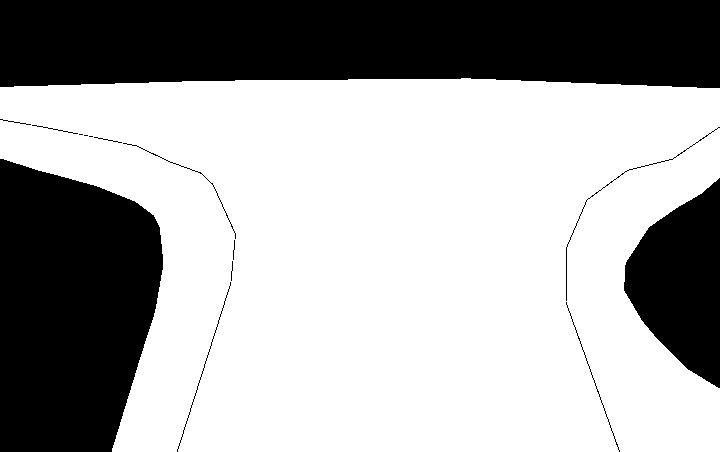
\includegraphics[width=\linewidth]{figures/generated/mixed_pln_1278_blue_green_display.png}
  \caption{Blue+green binary mask.}
\end{subfigure}
\caption[Example of the two binary conversions.]{Example of the two binary
conversions for \texttt{mixed\_pln\_1278}. In the lower masks, white denotes
traversable and black denotes untraversable. Blue-only retains the central raw
blue region; blue+green also admits the raw green shoulders. The upper raw red
field remains blocked in both policies.}
\label{fig:cat_binary_example}
\end{figure}

Figure~\ref{fig:cat_binary_example} also illustrates why the mapping must be
reported with every result. A binary visual can look plausible without
revealing whether green or red source regions were merged. The preprocessing
configuration therefore stores the traversable palette names and raw IDs, and
the processed summary records the mapping actually applied.

\section{Train, Validation, and Test Separation}

The original CaT test partition of 544 images is preserved intact and excluded
from gradient updates and automatic checkpoint selection. It is used for
read-only benchmark evaluation across several experiments, so it is not a
single-use blinded test set; Chapter~\ref{ch:protocols} states this limitation
explicitly. The original 1,268-image training partition is divided
into train and validation subsets by a deterministic hash:
\begin{equation}
 b(s)=
 \frac{
   \operatorname{int}\!\left(
   \operatorname{SHA256}\!\left(
     \operatorname{join}_{\texttt{:}}(\texttt{seed},\texttt{dataset},s)
   \right)_{0:12},16
   \right)}
 {16^{12}},
 \end{equation}
Here, $s$ is the complete sample identifier and $b(s)$ is its normalised hash
bucket, for which $0\leq b(s)<1$. The SHA-256 input is the UTF-8 string
$\operatorname{join}_{\texttt{:}}(\texttt{seed},\texttt{dataset},s)$, where
$\operatorname{join}_{\texttt{:}}$ concatenates the split seed, dataset name,
and complete sample identifier with colons. The subscript $0{:}12$ selects the
first 12 hexadecimal characters; $\operatorname{int}(\cdot,16)$ converts that
substring from base 16; division by $16^{12}$ normalises the integer to
$[0,1)$.
The sample is assigned to validation if $b(s)<0.2$. Split seed 1337 yields
1,002 training and 266 validation images. Hash bucketing makes the assignment
stable across machines and independent of filesystem ordering. It also
explains why the realised validation fraction is close to, but not exactly,
20\%.

Figure~\ref{fig:cat_data_partition} makes the information boundary explicit.
The validation set is created only from the official training part and is used
to select checkpoints. The official test branch remains outside optimisation
and automatic checkpoint selection, while repeated read-only evaluation is
shown as a separate benchmark path.

\begin{figure}[H]
\centering
\resizebox{0.94\textwidth}{!}{\begin{tikzpicture}[
  font=\sffamily\small,
  block/.style={draw,rounded corners=2pt,very thick,align=center,
    minimum height=1.22cm,inner sep=5pt},
  flow/.style={-{Latex[length=2.4mm]},very thick,draw=azulUC3M},
  sealed/.style={-{Latex[length=2.4mm]},very thick,dashed,draw=safety}
]
  \node[block,fill=softpurple,text width=2.15cm] (release) at (1.25,1.5)
    {\textbf{CaT release}\\1,812 images};
  \node[block,fill=softblue,text width=2.35cm] (dev) at (4.55,2.55)
    {\textbf{Official training part}\\1,268 images};
  \node[block,fill=safety!10,draw=safety,text width=2.25cm] (test) at (4.55,0.35)
    {\textbf{Official test}\\544 images};
  \node[block,fill=softorange,text width=2.55cm] (hash) at (8.0,2.55)
    {\textbf{Deterministic hash}\\development split};
  \node[block,fill=softgreen,text width=2.10cm,inner ysep=3pt] (train) at (11.35,4.10)
    {\textbf{Train}\\1,002 images\\update weights};
  \node[block,fill=softblue,text width=2.10cm,inner ysep=3pt] (val) at (11.35,1.75)
    {\textbf{Validation}\\266 images\\select checkpoint};
  \node[block,fill=safety!10,draw=safety,text width=2.25cm,inner ysep=3pt] (final) at (11.35,-0.60)
    {\textbf{Final evaluation}\\test once fixed};

  \draw[flow] (release) -- (dev);
  \draw[sealed] (release) -- (test);
  \draw[flow] (dev) -- (hash);
  \draw[flow] (hash) -- (train);
  \draw[flow] (hash) -- (val);
  \draw[sealed] (test) -- (final);

  \node[font=\footnotesize,align=center,text=safety] at (7.85,-1.88)
    {No test image is used to train weights or choose a checkpoint.};
\end{tikzpicture}
}
\caption[CaT train, validation, and test separation.]{CaT data separation used
throughout the thesis. Solid blue arrows describe development data flow; dashed
red arrows mark the preserved official test branch. Original schematic drawn
for this thesis.}
\label{fig:cat_data_partition}
\end{figure}

\begin{table}[H]
\centering
\caption{CaT split and the role of each subset.}
\label{tab:final_split}
\begin{tabularx}{\textwidth}{@{}lrrX@{}}
\toprule
\textbf{Split} & \textbf{Images} & \textbf{Share} & \textbf{Permitted use} \\
\midrule
Train & 1,002 & 55.30\% & Gradient-based weight optimisation \\
Validation & 266 & 14.68\% & Epoch checkpoint selection by mIoU \\
Test & 544 & 30.02\% & Read-only benchmark scoring; no training or checkpoint selection \\
\midrule
Total & 1,812 & 100.00\% & \\
\bottomrule
\end{tabularx}
\end{table}

Table~\ref{tab:final_split} records the exact image counts and prevents the
roles of validation and test data from being conflated later in the thesis.

Every processed sample is entered in a JSON manifest with its split, sample
identifier, processed RGB path, processed mask path, label source, and raw
label path. Training and evaluation read this manifest rather than rediscovering
files. The manifest therefore acts as the contract between preprocessing and
all subsequent experiments.

\section{Image and Mask Preparation}

The training loader applies a small, explicit sequence of operations:
\begin{enumerate}
  \item open the processed RGB file and convert it to three-channel RGB;
  \item open the binary mask without colour conversion;
  \item resize the image to the configured width and height with bilinear
  interpolation;
  \item resize the mask with nearest-neighbour interpolation;
  \item if training augmentation is enabled, apply a matched horizontal flip
  and image-only photometric transforms;
  \item convert RGB values to floating point in $[0,1]$, transpose to
  channel-first format, and convert mask values to integer class IDs.
\end{enumerate}

Nearest-neighbour mask interpolation is essential. Bilinear interpolation
would produce fractional values at class boundaries and turn a categorical
label map into an unintended soft target. All controlled experiments use a
resolution of $640\times384$. This converts the different native image sizes
to one tensor shape, supports batching, and is divisible by the main
architectures' downsampling factors. Resizing changes the aspect ratio
slightly because the native ratios are not identical. Crop-and-pad
preprocessing was considered but not used, so this small distortion is part of
the declared protocol.

PIDNet-S and the other ordinary controlled models consume the $[0,1]$ tensor
directly; no ImageNet mean or standard-deviation normalisation is applied by
the common loader. ROD receives the same tensor, then internally resizes it to
$1024\times1024$ and applies the ImageNet mean
$[0.485,0.456,0.406]$ and standard deviation
$[0.229,0.224,0.225]$ expected by EfficientSAM. This model-specific operation
is described separately because it changes ROD's computation even though its
external input remains $640\times384$.
The mean and standard-deviation entries are ordered red, green, blue.

When enabled, augmentation uses deterministic per-sample randomness derived
from the seed, sample index, and epoch. The tested recipe consists of:
\begin{itemize}
  \item horizontal flip with probability 0.5;
  \item brightness, contrast, and saturation factors sampled independently
  from $[0.9,1.1]$;
  \item sharpness adjustment with probability 0.25 and factor $[0.7,1.3]$;
  \item Gaussian blur with probability 0.2 and radius $[0.2,1.1]$.
\end{itemize}
Bracketed augmentation intervals are uniform sampling ranges. Colour and
sharpness factors are dimensionless multipliers, whereas blur radius is
measured in pixels.
Only the horizontal flip changes the mask. The reference PIDNet checkpoint
disables this entire recipe after the controlled ablation showed lower
validation-selected test performance when it was enabled. This result applies
to the stated recipe, not to augmentation in general.

\section{Common Software Workflow}

The repository separates dataset audit, preprocessing, training, evaluation,
qualitative review, inference export, and benchmarking into configuration-driven
entry points. Figure~\ref{fig:common_pipeline} shows the lifecycle. The
separation was chosen so that evaluating a saved checkpoint does not
implicitly retrain it and so that a benchmark can name the exact model and
processed manifest it consumes.

\begin{figure}[H]
\centering
\resizebox{\textwidth}{!}{\begin{tikzpicture}[
  node distance=0.52cm,
  pipestep/.style={draw,rounded corners=2pt,text width=2.3cm,minimum height=1.15cm,
    align=center,font=\small,inner sep=4pt},
  artifact/.style={draw,dashed,rounded corners=2pt,text width=2.2cm,minimum height=0.75cm,
    align=center,font=\footnotesize,inner sep=3pt},
  arrow/.style={-{Latex[length=2.3mm]},thick,draw=azulUC3M}
]
\node[pipestep,fill=softblue] (audit) {\textbf{Audit}\\pair RGB, palette mask, integer map};
\node[pipestep,fill=softgreen,right=of audit] (map) {\textbf{Convert}\\apply policy; write binary mask};
\node[pipestep,fill=softorange,right=of map] (split) {\textbf{Split}\\hash development set; preserve test};
\node[pipestep,fill=softpurple,right=of split] (load) {\textbf{Load}\\resize, scale, optional augmentation};
\node[pipestep,fill=softblue,below=1.75cm of load] (train) {\textbf{Train}\\optimise; validate each epoch};
\node[pipestep,fill=softgreen,left=of train] (select) {\textbf{Select}\\highest validation mIoU};
\node[pipestep,fill=softorange,left=of select] (eval) {\textbf{Evaluate}\\fixed threshold; aggregate confusion};
\node[pipestep,fill=softpurple,left=of eval] (review) {\textbf{Review and deploy}\\rank cases; benchmark};
\draw[arrow] (audit) -- (map);
\draw[arrow] (map) -- (split);
\draw[arrow] (split) -- (load);
\draw[arrow] (load) -- (train);
\draw[arrow] (train) -- (select);
\draw[arrow] (select) -- (eval);
\draw[arrow] (eval) -- (review);

\node[artifact,below=0.2cm of map] (manifest) {binary masks + manifest};
\node[artifact,below=0.2cm of select] (checkpoint) {\texttt{best.pt}};
\node[artifact,below=0.2cm of review] (reports) {metrics, figures, timing JSON};
\draw[arrow,dashed] (map) -- (manifest);
\draw[arrow,dashed] (select) -- (checkpoint);
\draw[arrow,dashed] (review) -- (reports);
\end{tikzpicture}
}
\caption[Common implementation workflow.]{Common implementation workflow from
raw CaT files to saved evidence. Dashed boxes are persistent artifacts that
allow a reported result to be traced to its data, selected checkpoint, and
evaluation outputs.}
\label{fig:common_pipeline}
\end{figure}

During training, the data loader shuffles only the training subset. Validation
is deterministic and unaugmented. At the end of each epoch the model is
evaluated on all 266 validation images; \texttt{best.pt} is replaced only if
validation mIoU improves. The checkpoint stores the model state, optimiser
state, epoch, complete configuration, and class weights. The test evaluator
loads that checkpoint, switches the model to evaluation mode, disables
gradients, iterates through the test manifest without shuffling, and
accumulates one $2\times2$ confusion matrix.

The output directory for each experiment contains the training history,
\texttt{best.pt}, \texttt{last.pt}, validation visualisations, test metrics,
and selected review panels. Generated repeat-seed configurations are retained
instead of being assembled only in memory. These decisions make the
experimental procedure inspectable after training hardware is no longer
available.

\section{Annotation Ambiguity and Observable Evidence}
\label{sec:annotation_ambiguity}

For metric computation the CaT mask is ground truth: every disagreement is
counted as model error. For scientific interpretation, however, the annotation
is a human judgement about vehicle capability from a scene. Several cases show
why disagreement cannot always be diagnosed from RGB appearance alone.

In \texttt{mixed\_pln\_1278}, the annotated blue corridor continues through a
pale open area, while the cultivated field at the top of the image is
off-road-only and therefore blocked by the blue+green policy. The field and
track share colour and texture cues in the RGB image. The label may depend on
surface preparation, soil support, crop rows, or the intended route---physical
information that a single frame does not establish.

In \texttt{mixed\_118}, the RGB frame shows dense woodland and a leaf-covered
floor with almost no visually distinct road edge. The annotation nevertheless
assigns a broad, irregular foreground region to the sedan-capable class. Some
of that region may correspond to a faint route visible to the annotator or in
adjacent frames, but its extent is difficult to reconstruct from this image
alone.

\begin{figure}[H]
\centering
\begin{subfigure}[t]{0.485\linewidth}
  \centering
  \includegraphics[width=\linewidth]{../CAT/mixed/Test/imgs/img_pln_1278.png}
  \caption{\texttt{mixed\_pln\_1278}: RGB image.}
\end{subfigure}\hfill
\begin{subfigure}[t]{0.485\linewidth}
  \centering
  \includegraphics[width=\linewidth]{../CAT/mixed/Test/annos/anno_pln_1278.jpg}
  \caption{\texttt{mixed\_pln\_1278}: released annotation.}
\end{subfigure}

\vspace{0.20cm}
\begin{subfigure}[t]{0.485\linewidth}
  \centering
  \includegraphics[width=\linewidth]{../CAT/mixed/Test/imgs/img_118.png}
  \caption{\texttt{mixed\_118}: RGB image.}
\end{subfigure}\hfill
\begin{subfigure}[t]{0.485\linewidth}
  \centering
  \includegraphics[width=\linewidth]{../CAT/mixed/Test/annos/anno_118.jpg}
  \caption{\texttt{mixed\_118}: released annotation.}
\end{subfigure}
\caption[Examples of ambiguity in the available RGB evidence.]{RGB frames and
released CaT annotations for the two cases discussed in the text. In
\texttt{mixed\_pln\_1278}, the pale track and cultivated field have similar
appearance despite different capability labels. In \texttt{mixed\_118}, dense
vegetation and leaf-covered ground provide few clear cues for the broad
accepted foreground region. The annotation colours retain the
original four-class CaT vehicle-capability hierarchy.}
\label{fig:cat_ambiguity_examples}
\end{figure}

Figure~\ref{fig:cat_ambiguity_examples} places the two discussed RGB frames
beside their released annotations so that the ambiguity is visible rather than
asserted only in prose.

In \texttt{mixed\_459}, low vegetation and the track meet along an irregular
foreground edge. Moving the line by several pixels changes the boundary-band
score substantially even though more than one contour may appear plausible
from RGB alone.

These examples do \emph{not} demonstrate that the annotations are wrong. The
annotator may have had route knowledge, higher-resolution context, or a
vehicle-capability convention unavailable in the displayed frame. Conversely,
visual plausibility does not prove physical traversability. CaT provides
neither multiple independent annotations nor inter-annotator agreement, so the
amount of label uncertainty cannot be estimated from the released data. The
thesis can identify cases where RGB evidence is insufficient to justify a
precise boundary, but it cannot calculate a noise rate or replace the supplied
label with a preferred alternative.

This limitation affects both training and evaluation. The model is optimised
to reproduce the annotations, and the reported FSR/FBR describe disagreement
with that policy. They are not direct measurements of real vehicle incidents.
The qualitative chapter therefore distinguishes clear spatial model failures
from cases whose physical status would require additional evidence.
